\documentclass[12pt]{article}
\usepackage[top=1in, bottom=1in, left=1in, right=1in]{geometry}
\usepackage[justification=centering]{caption}
\usepackage{graphicx}
\usepackage{listings}
\usepackage{color}
\usepackage{indentfirst}
\usepackage{hyperref}
\usepackage{siunitx}
\usepackage{float}
\usepackage{amsmath}

\lstset{ %
	%language=C,                % choose the language of the code
	basicstyle=\scriptsize,       % the size of the fonts that are used for the code
	                  % how far the line-numbers are from the code
	backgroundcolor=\color{white},  % choose the background color. You must add \usepackage{color}
	showspaces=false,               % show spaces adding particular underscores
	showstringspaces=false,         % underline spaces within strings
	showtabs=false,                 % show tabs within strings adding particular underscores
	%frame=single,           % adds a frame around the code
	tabsize=2,          % sets default tabsize to 2 spaces
	captionpos=b,           % sets the caption-position to bottom
	breaklines=true,        % sets automatic line breaking
	breakatwhitespace=false,    % sets if automatic breaks should only happen at whitespace
	escapeinside={\%*}{*)}          % if you want to add a comment within your code
}

\begin{document}
\title{Microprocessor Systems\\ Lab 4: Analog Conversion \&\ MAC }
\author{Nick Choi \and Samuel Deslandes}
\date{10/31/16}
\maketitle
\pagebreak
\section{Introduction}

The overall goal of this lab is to become familiar with configuring the ADC, DAC and MAC on the 8051 to perform various applications such as digital filtering and implementing a voltmeter. 

The lab is divided into three sections. In the first section, a C program is created to configure the ADC on the 8051 to convert analog signals to digital signals when a pushbutton is pressed. The code polls a flag which is set when the pushbutton is pressed to determine whether or not to initialize an analog to digital conversion. When a conversion has been completed, the program displays the digital voltage reading rounded to six decimal places as well as the minimum voltage, maximum voltage and a moving average of the last 16 voltage readings via the ANSI terminal. The output is updated each time a conversion takes place. 

In the third section, a C program is created to configure the DAC on the 8051 to convert digital signals to analog signals. This section builds upon the code in section 1 because the output of the ADC is used as the input of the DAC. The output of the DAC was observed using an oscilloscope. 

In the fourth section, a new C program is written to implement an infinite impulse response (IIR) filter using the MAC on the 8051. The inputs of the digital filter are the present analog reading, the past two analog readings and the last digital output of the filter. All of these inputs are scaled by a coefficient and added together to reconstruct an analog waveform with digital signals using the 8051’s MAC. The output of the filter was observed using an oscilloscope. 

\section{Methods}
\subsection{Software}
The code for parts 1, 2 and 3 can be found in the appendix below. All code was uploaded and run on the 8051 through the programming/debugging USB port. 

\subsubsection{Part 1}

The purpose of this program is to create a digital voltmeter using the analog to digital converter (ADC) on the 8051. When the pushbutton is pressed, an A-D conversion begins, and the result is used to calculate a voltage which is then displayed on the terminal. 

Configurations for the ADC can be found in the REFOCN, ADC0CF, and ADC0CN registers, as well as the AMX0SL and AMX0CF registers for selecting the mode of operation of the analog input pins and which pins are selected for use. In the REF0CN SFR, bit1 enables the bias generator; this must be enabled. Bit0 of this SFR enables the internal reference buffer, which sets VREF0 to 2.4V. When using an external voltage source as a reference, this bit should be disabled. For this section the internal voltage reference was used. For the purposes of this lab, only one analog input operating in single-ended mode was needed, therefore the AMX0SL and AMX0CF registers did not require any modification; using the reset (default) values of these SFRs results in AIN0.0 selected with the desired mode of operation. The ADC0CF SFR, sets the gain for the input voltage (AIN0.0) and the sampling rate for the conversion process. The sampling rate can be calculated as a function of SYSCLK and the value loaded into AD0SC (bit3-bit7 of this SFR) using the following equation:
\begin{align*}
AD0SC = \frac{SYSCLK}{2\times CLK_{SAR0}}-1\\
\text{where $CLK_{SAR0}$ is the ADC sampling rate.}
\end{align*}
\noindent
Bits0-2 of this SFR are used to set the gain. For this lab a gain of 1 was used with AD0SC set to 23, resulting in an $SAR_{CLK}$ of approximately \si{1}{MHz}. Lastly ADC0 must be enabled via bit7 of the ADC0CN, which is also bit addressable as AD0EN.

For starting conversions, the pushbutton was connected as an external interrupt source as was previously done in lab 2. To do this, /INT0 must be routed to a port pin (P0.2 in this case) via the crossbar (XBR1) and external interrupts must be enabled. This can be done by setting the EA and EX0 bit addresses. Because only one conversion per button press was desired, /INT0 was set to be triggered on a negative falling edge by setting the IT0 bit address.

UART0 was also used to display the output onto the terminal, which is enabled in the XBR0 SFR. For configuring the ports, TX (P0.0) must be configured for push-pull, and RX (P0.1) and /INT0 (P0.2) must be set for open-drain with high impedance. This can be set in the P0MDOUT and P0 SFRs.

The code for this section follows a simple routine in which the program waits for a flag set by the /INT0 ISR to go high. This starts an A-D conversion, and the result is then used to calculate a voltage which is then printed to the terminal along with various statistics. Before starting the A-D conversion, the conversion complete interrupt flag (AD0INT) must be cleared; as its name implies, this bit is set by the hardware once the conversion is completed. To begin the conversion, set the AD0BUSY, then wait for the conversion to be completed by polling AD0INT. At this point the result of the conversion can be obtained by reading the 16bit SFR ADC0. The result of the conversion is the ratio of the input voltage between 0 and VREF0 mapped to a value between 0 and 4095. The result can be converted back into a voltage using the following equation:
\begin{align*}
V_{in} = \frac{ADC0}{4096} \times VREF0\\\text{where $VREF0 =$ 2.4\si{V}}
\end{align*}

In order to display the max, min, and average voltage over the past 16 samples each value is stored in an array of integers of size 16. When the array is filled, using modular arithmetic the oldest entry in the array is updated with the newest sample. Using this array the max, min, and average can easily be calculated by traversing the array. Once these statistics have been calculated, the voltage values are displayed in decimal form, along with the raw result of the conversion displayed in hex. 

\subsubsection{Part 3}

The program for this section follows a simple routine in which the result of an A-D conversion is sent directly to the DAC to be converted back to an analog signal. 

The initialization for the ADC was similar to the previous section, the only difference being that VREF0 is now defined by an external \si{3}{V} voltage source. To do this, bit0 of the REF0CN register must be cleared. Once REF0CN is configured, the only initialization necessary for DAC0 is setting bit7 of the DAC0CN register; this enables the DAC0 output pin.

The routine for this program continuously performs A-D conversions, and  outputs the result to the DAC by loading it into the 16bit SFR ``DAC0''.

\subsubsection{Part 4}

The code for this section follows a similar procedure to that of the previous section, while introducing the MAC to implement a digital filter. As was done previously, an analog input is read in using the ADC, the result is passed through the filter, and the filtered result is then output through the DAC.

The IIR filter used can be described by the following difference equation:
\begin{gather*}
y(k) = 0.31250000x(k) + 0.31250000x(k-2) + 0.24038462x(k-1) + 0.29687500y(k-1)\\
\text{where y(k) is the current output}\\
\text{y(k-1) is the previous output}\\
\text{x(k) is the current sample}\\
\text{x(k-1) is the previous sample}\\
\text{and x(k-2) is the sample before the previous sample}
\end{gather*}

After the analog input was read in through the ADC, the variables storing the previous sample values were updated, and an offset value was subtracted from the current sample. This was needed because the function generator input was set to a \si{3}{Vpp} wave with a \si{\num{1.5}}{V} offset such that the wave ranged from \si{0-3}{V}.

Next, the accumulator was cleared, and the MAC was set to operate in integer multiply-accumulate mode. This can be set in the MAC0CF SFR. At this point, values can be loaded into the MAC. Since the MAC was operating in integer mode, the coefficients were multiplied by a large constant ($2^{10}$); the final result was normalized in the accumulator via right bit-shift operations once the calculations were complete.    

First, the MAC0A register was loaded with the decimal value 320 ($0.3125\times 2^{10}$), then MAC0BH loaded with the high 8 bits of the current sample and MAC0BL with the lower 8 bits of the current sample. This represented the $0.31250000x(k)$ portion of the above difference equation. Next, MAC0BH and MAC0BL were similarly loaded with the sample before the previous sample, representing the $0.31250000x(k-1)$ portion of the equation. After this, MAC0A was loaded with the decimal value 246 ($\approx 0.24038462\times 2^{10}$), and MAC0BH and MAC0BL with the previous sample, representing $0.24038462x(k-1)$. Lastly, MAC0A was loaded with the 304 ($0.296875\times 2^{10}$), and MAC0BH and MAC0BL with the previous output, representing the final part of the equation $0.29687500y(k-1)$. These products are summed in the accumulator and as mentioned before, were normalized by performing 10 right bit-shit operations. This was accomplished using a for loop and setting the ``MAC0CF'' register to \texttt{0x30}; this executes a single shift of the value in the accumulator to the right.

Values are stored in the accumulator using 5 8bit registers, ``MAC0ACC0'' - ``MAC0ACC3'' and an overflow register ``MAC0OVR''. After the bit-shift operations, the desired result can be found in registers ``MAC0ACC0'' and ``MAC0ACC1''. The values in these registers were combined into a single 16bit variable and the offset originally subtracted from the current sample is added back in. The final result is then output to DAC0.
\subsection{Hardware}

The hardware for section 1 involved using the potentiometer module to vary the voltage input to AIN0.0 for the A-D conversions. Rather than using the pins on the 60pin bus, the Analog I/O terminal block (J20) was used. A schematic for this can be viewed in the appendix below. The output of the potentiometer was connected to pin 5 on the terminal block (AIN0.0), and pin 8 (AGND) was connected to a common ground on the board. 

Section 3 called for the use of a function generator and an oscilloscope, as well as an external voltage source for VREF0. The \si{3}{V} reference voltage was generated using the potentiometer module, and was connected to pin 7 on the terminal block (VREF0). The function generator was set to produce a \si{3}{Vpp} sinusoidal wave with \num{1.5}\si{V} offset. This was connected to AIN0.0 on the terminal block (pin 5) using an alligator clip. The output from DAC0 (pin 3 on the terminal block) was connected to the oscilloscope also using an alligator clip. As was done before, AGND was connect to a universal ground. A schematic for this can be viewed in the appendix section below. 

The hardware for section 4 was identical to that of the previous section. 

\section{Results}

By completing section one of the lab, a C program was developed to convert variable analog voltages to digital values used to calculate a digital voltage. The program displayed the converted voltages, as well as statistics including the moving average of the last 16 samples, and the min/max voltage values. After completing section three of the lab, a C program was developed to convert digital voltages obtained from an ADC to the equivalent analog voltage values. By completing section four of the lab, a C program was created to use the MAC on the 8051 to reconstruct analog signals using the ADC and DAC written for the previous sections of the lab. The output of the MAC represented the output of an infinite impulse response digital filter.


\section{Conclusion}


The end results of the lab generally matched with the initial goals however there were numerous instances where the system did not behave as expected. In section 4 of the lab, the output of our digital filter was only able to accurately reconstruct the analog input signal up to a certain frequency threshold. This anomaly can be explained by the Nyquist sampling theorem which states that in order to accurately represent an analog signal, the sampling frequency must be at least double the frequency of the input signal. If the sampling frequency falls below this threshold, the 8051 is unable to obtain enough samples to accurately model the input waveform. In this lab, the output signal did not accurately represent the input waveform after 25 kHz. Given that the sampling frequency for the 8051 was calculated to be 50 kHz, this result is what could be expected. 

Prior to implementing the filter with the 8051\textquoteright s MAC, a software implementation of the IIR filter was used to make it easier to debug this section of the lab. Although the output signals of the software implementation are generally the same as the MAC, the algorithm\textquoteright s performance is limited compared to the MAC counterpart. This is because the code takes longer to compute the output values than the MAC due to the innate latency involved with running the code. 

If more time was given to complete this lab assignment, the voltmeter created in section one would be modified to achieve the functionalities described in section two of the lab. This would create a digital voltmeter which would be capable of measuring the frequency of input waveforms as well as the AC RMS voltage value of the signal. 



\pagebreak
\section{Appendices}
\subsection{Analog I/O Terminal block}
	\begin{figure}[H]
		\centering
		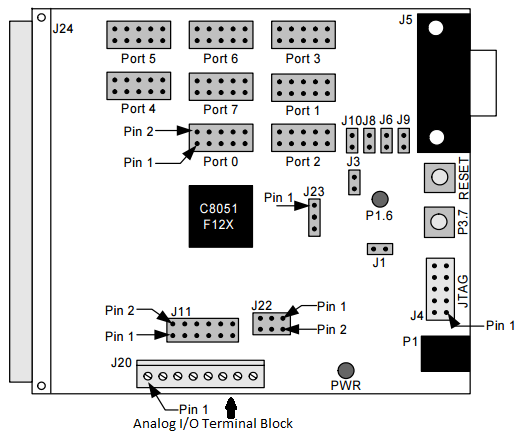
\includegraphics[]{board.png}
		\caption{C8051F120 Targer Board layout}
		\label{board layout}
	\end{figure} 
	\begin{table}[h]
		\centering
		\begin{tabular}{|l|l|}
			\hline
			Pin\# & Description \\ \hline
			1 & CP0+\\ \hline
			2 & CP0-\\ \hline
			3 & DAC0\\ \hline
			4 & DAC1\\ \hline
			5 & AIN0.0\\ \hline
			6 & AIN0.1\\ \hline
			7 & VREF0\\ \hline
			8 & AGND (Analog Ground)\\ \hline
		\end{tabular}
		\caption{J20 Terminal Block reference table}
		\label{refTable}
	\end{table}
\subsection{Modified putget.h}
	\lstinputlisting{putget.h}
\subsection{Part 1}
	\subsubsection{Circuit Schematic for section 1}
		\begin{figure}[H]
			\centering
			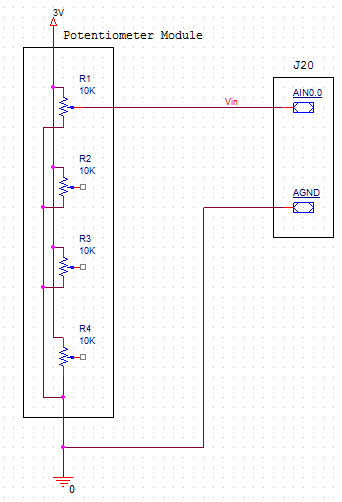
\includegraphics[]{Part1.png}
			\caption{Circuit schematic for part 1}
			\label{schematic1}
		\end{figure} 
		\pagebreak
	\subsubsection{Code for part 1}
		\lstinputlisting{part1-2.c}
\subsection{Schematic for parts 3 and 4}
	\begin{figure}[H]
		\centering
		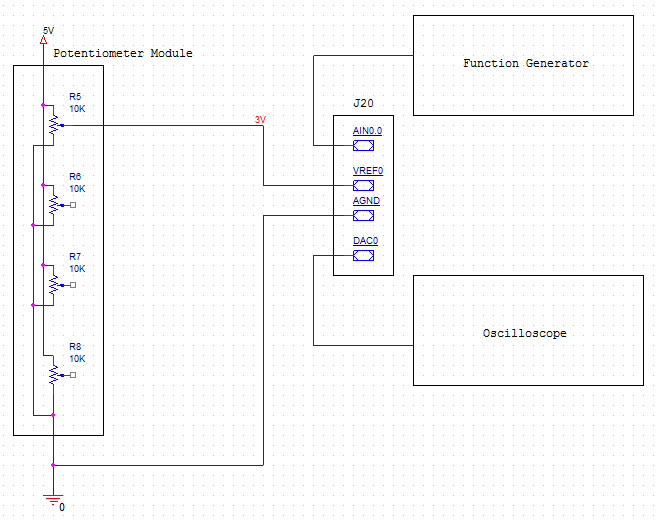
\includegraphics[]{Part2.png}
		\caption{Circuit schematic for part 2}
		\label{schematic2}
	\end{figure} 
\subsection{Part 3}
	\subsubsection{Code for part 3}
		\lstinputlisting{part3.c}	

%\pagebreak
\subsection{Part 4}
	\subsubsection{Code for part 4}
		\lstinputlisting{part4-2.c}
	
\section{References} 
\noindent
``MPS Lab 4,'' in RPI ECSE Department, 2016. [Online]. Available: \url{http://www.rpi.edu/dept/ecse/mps/MPS_Lab_Ex4-ADC.pdf}. Accessed: Oct. 30, 2016.\\
\newline\noindent
``C8051 Manual,'' in RPI ECSE Department, 1.4 ed., 2005. [Online]. Available: \url{https://www.ecse.rpi.edu/courses/CStudio/Silabs/C8051F12x-13x.pdf}. Accessed: Oct. 30, 2016.\\
\newline\noindent
``C8051F12x Development Kit User's Guide ,'' in RPI ECSE Department, Rev. 0.6,May 2005. [Online]. Available: \url{https://www.ecse.rpi.edu/courses/CStudio/Silabs/C8051F12x-DK.pdf}. Accessed: Oct. 30, 2016.







\end{document}